\documentclass{article}

% Packages:
\usepackage{geometry}
\usepackage{graphicx}
\usepackage{amsmath}
\usepackage{tikz}
\usepackage{float}

% Settings:
\setlength{\parindent}{0pt}


\begin{document}

\title{WALT}
\author{Your Name}
\date{\today}

\maketitle

\section{Objective}

The objective of this project is to design, develop, and implement a wheeled quadruped robot capable of performing autonomous navigation in a controlled environment. The robot will integrate both walking and driving capabilities, allowing it to:

\begin{enumerate}
    \item Drive fully autonomously in a controlled environment from a start to an end point.
    \item Detect and avoid obstacles autonomously while maintaining a smooth path.
    \item Climb or overcome obstacles that hinder passing.
    \item Switch between driving and walking modes based on environmental conditions, such as encountering an obstacle that requires climbing.
\end{enumerate}

This project aims to combine real-time sensor data processing (e.g., LIDAR, cameras) with intelligent decision-making algorithms to allow the robot to autonomously navigate complex paths. Moreover, the robot has to be designed, and a sophisticated selection of the hardware components (such as servos, microcontroller, sensors, etc.) is necessary. Particular emphasis is placed on the development of a control system to manage locomotion and walking gaits, ensuring that all elements are combined effectively into a unified embedded system.

\subsection{Target Route}

The target route for the robot is designed to test its ability to navigate both driving and climbing modes in a structured environment. The route goes through a corridor, includes dynamic obstacle avoidance, and ends with a climbing task. Below is a detailed breakdown of the route and its key features:

\begin{enumerate}
    \item \textbf{Start:} The robot begins at the designated Start Point, located in a corridor.
    \item \textbf{Driving along the corridor:} The robot drives fully autonomously through the aisle and should be able to navigate past various obstacles.
    \item \textbf{Turning in the corridor:} After navigating the horizontal aisle, the robot should be able to navigate safely around a corner in the corridor.
    \item \textbf{Climbing an Obstacle:} To test and demonstrate the robot's climbing and walking capabilities, it will encounter an obstacle that requires a transition from driving mode to walking/climbing mode.
    \item \textbf{Goal:} After successfully completing the route, the robot reaches a predefined endpoint.
\end{enumerate}

This route evaluates the robot's capabilities in obstacle detection and avoidance, control and mechanical design, seamless transitions between driving and walking modes, and successfully overcoming challenges to reach the predefined endpoint.

\begin{figure}[h!]
    \centering
    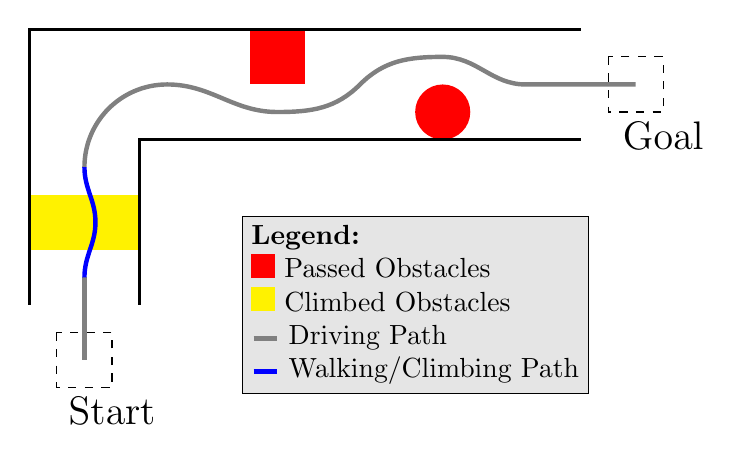
\begin{tikzpicture}[scale=0.7]

    % Obstacles
    \fill[red] (-6,-1) rectangle (-5,0);
    \fill[red] (-2.5,-1.5) circle (0.5);
    \fill[yellow] (-10,-4) rectangle (-8,-3);
    
    % Walls
    \draw[very thick] (0,0) -- (-10,0) -- (-10,-5);
    \draw[very thick] (0,-2) -- (-8,-2) -- (-8, -5);
    
    % Start
    \draw [black,dashed] (-9.5,-5.5) rectangle (-8.5,-6.5) node [black,below] {\Large Start};
    
    % Goal
    \draw [black,dashed] (0.5,-0.5) rectangle (1.5,-1.5) node [black,below] {\Large Goal};
    
    % Driving Path
    \draw [gray, ultra thick] (1,-1) % Draws a line
      to [out=180,in=0] (-1,-1) %Line
      to [out=180,in=0] (-2.5,-0.5) %Arc
      to [out=180,in=45] (-4,-1) %Arc
      to [out=225,in=0] (-5.5,-1.5) %Arc
      to [out=180,in=0] (-7.5,-1) %Arc
      to [out=180,in=90] (-9,-2.5) %Arc
      ;
    \draw[gray, ultra thick] (-9,-4.5) -- (-9,-6);
    
    % Walking Path
    \draw [blue,ultra thick] (-9,-2.5)
    to [out=270,in=90] (-8.8,-3.5)
    to [out=270,in=90] (-9,-4.5)
    ;

    % Legend
    \node[draw, fill=gray!20, minimum width=4cm, minimum height=2cm, align=left] (notationBox) at (-3,-5) {
    \textbf{Legend:} \\ 
    \tikz\fill[red] (0,0) rectangle (0.3cm,0.3cm); Passed Obstacles\\
    \tikz\fill[yellow] (0,0) rectangle (0.3cm,0.3cm); Climbed Obstacles\\
    \tikz[baseline=-0.5ex]\draw[gray, ultra thick] (0,0) -- (0.3,0); Driving Path\\
    \tikz[baseline=-0.5ex]\draw[blue, ultra thick] (0,0) -- (0.3,0); Walking/Climbing Path
    };
    
    \end{tikzpicture}
    \caption{Target route of the robot}
    \label{fig:Target_Route}
\end{figure}

\subsection{Real-World Application of the Project}

The quadruped robot is well-suited for a variety of real-world applications. It excels in autonomous delivery, particularly for last-mile logistics, where fast-paced driving on flat surfaces is required, but the ability to overcome obstacles, such as stairs or curbs, is essential. In industrial environments, such as factories and warehouses, the robot is ideal for navigating primarily flat surfaces at high speeds while still being capable of overcoming occasional obstacles, ensuring smooth and efficient operations. Its versatility makes it valuable in any environment where fast driving is the primary mode of transport, but the ability to switch to walking or climbing is mandatory to handle challenging obstacles.

\section{Project Structure and Task Allocation}

The figure below illustrates the hierarchical structure and flow of data and control signals within the quadruped robot system. The system is organized into five primary components:

\begin{enumerate}

    \item \textbf{Perception}: This module, operating within a laptop environment, processes sensor data (such as from a camera or a LIDAR) to generate a live feed of the robot’s surroundings, such as detected objects or walls. The processed data is essential for decision-making in autonomous navigation.
    
    \item \textbf{Path Planning}: Based on the perception data, the path planning algorithm calculates optimal routes, avoiding obstacles while ensuring smooth navigation. This algorithm also runs on a laptop.
    
    \item \textbf{Electronics and Microcontroller}: This component is responsible for executing commands from the path planning module, handling low-level operations like motor control, sensor interfacing, and communication with the perception system.
    
    \item \textbf{Control}: The control system takes high-level decisions from the electronics and microcontroller and translates them into commands for the actuators, ensuring stable and effective locomotion.
    
    \item \textbf{Mechanical Design and Structure}: This section is responsible for the physical movement and interaction of the robot with its environment, based on commands from the control system.
\end{enumerate}
    
The live feed loop allows continuous feedback from the robot to the perception system, enabling real-time adjustments and efficient decision-making in dynamic environments.


\begin{figure}[H]
    \centering
    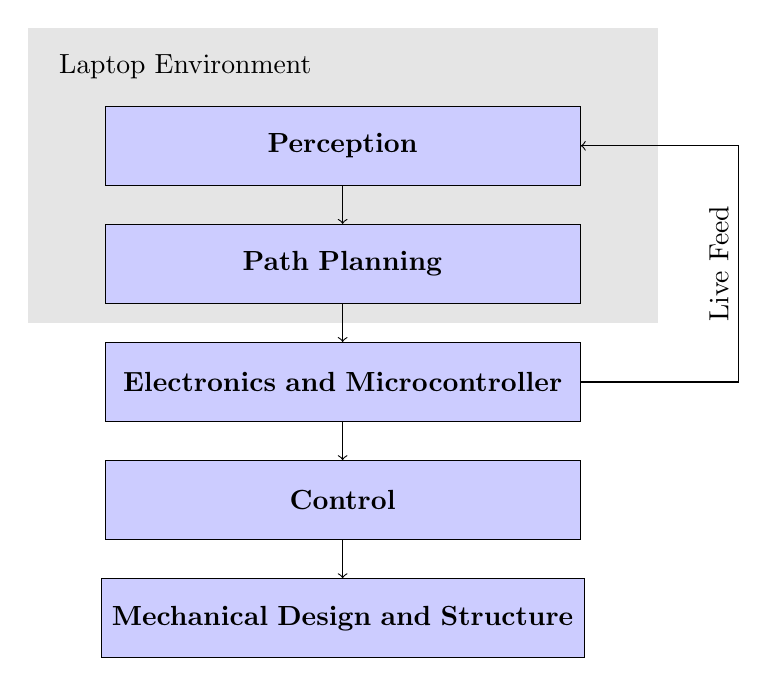
\begin{tikzpicture}
    
    % Laptop Environment
    \fill[gray!20] (-4, 1.5) rectangle (4, -2.25);
    \node at (-2, 1) {Laptop Environment};

    % Perception:
    \node[draw, fill=blue!20, minimum width=6cm, minimum height=1cm, text width=5.8cm, align=center] (Perception) at (0, 0) {
    \textbf{Perception}
    };

    % Path Planning
    \node[draw, fill=blue!20, minimum width=6cm, minimum height=1cm, text width=5.8cm, align=center] (Path Planning) at (0, -1.5) {
    \textbf{Path Planning}
    };

    % Electronics and Microcontroller
    \node[draw, fill=blue!20, minimum width=6cm, minimum height=1cm, text width=5.8cm, align=center] (Electronics) at (0, -3) {
    \textbf{Electronics and Microcontroller}
    };

    % Control:
    \node[draw, fill=blue!20, minimum width=6cm, minimum height=1cm, text width=5.8cm, align=center] (Control) at (0, -4.5) {
    \textbf{Control}
    };

    % Mechanical Design and Structure
    \node[draw, fill=blue!20, minimum width=6cm, minimum height=1cm, text width=5.9cm, align=center] (Mechanical) at (0, -6) {
    \textbf{Mechanical Design and Structure}
    };

    % Connections
    \draw[->] (Perception.south) -- (Path Planning.north);
    \draw[->] (Path Planning) -- (Electronics);
    \draw[->] (Electronics) -- (Control);
    \draw[->] (Control) -- (Mechanical);
    \draw[->] (Electronics.east) -- ++(2cm, 0) |- (Perception.east)node[pos=0.25, above, rotate=90] {Live Feed};

    \end{tikzpicture}
    \caption{Project Structure}
    \label{fig:Project_Structure}
\end{figure}

\end{document}
